\section{Przedstawienie danych statystycznych}

\begin{frame}{Struktura mocy zainstalowanej w Polsce z podziałem na typy elektrowni (stan na 31.12.2024)}
    \includetable{installed_capacity}
\end{frame}

\begin{frame}{Struktura mocy zainstalowanej w Polsce na 31.12.2024}
    \includefigure{installed_power_structure}
\end{frame}

\begin{frame}{Moc zainstalowana w Polsce na przestrzeni lat [MW]}
    \begin{center}
    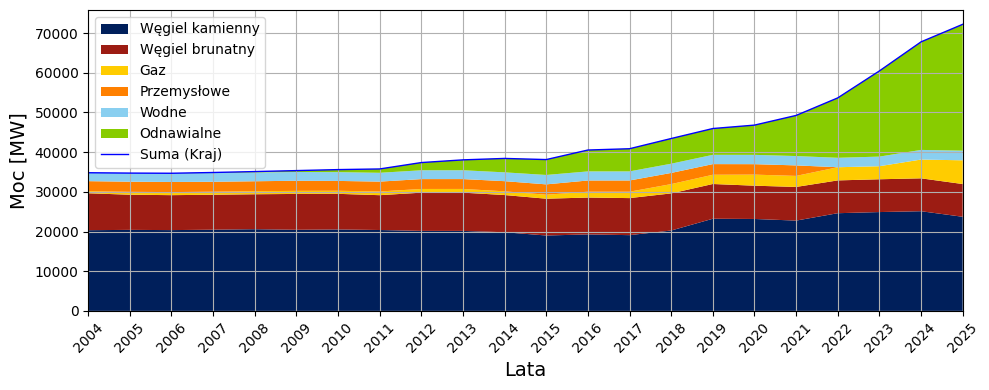
\includegraphics[width=0.8\linewidth]{images/powerOverYears.png}
    \end{center}
    \begin{itemize}
    \item W ostatnich latach można zauważyć bardzo szybki przyrost mocy zainstalowanej w postaci źródeł odnawialnych.
    \item OZE stanowią obecnie zdecydowanie najprężniej rozwijający się rodzaj źródeł energii w Polsce.
    \end{itemize}
\end{frame}

\begin{frame}{Udział OZE i energii nuklearnej w sumarycznej produkcji energii wybranych krajów europejskich (2023)}
    \includetable{OZE_percentage}
\end{frame}

\begin{frame}{Udział OZE i energii nuklearnej w sumarycznej produkcji energii wybranych krajów europejskich (2023)}
    \begin{center}
    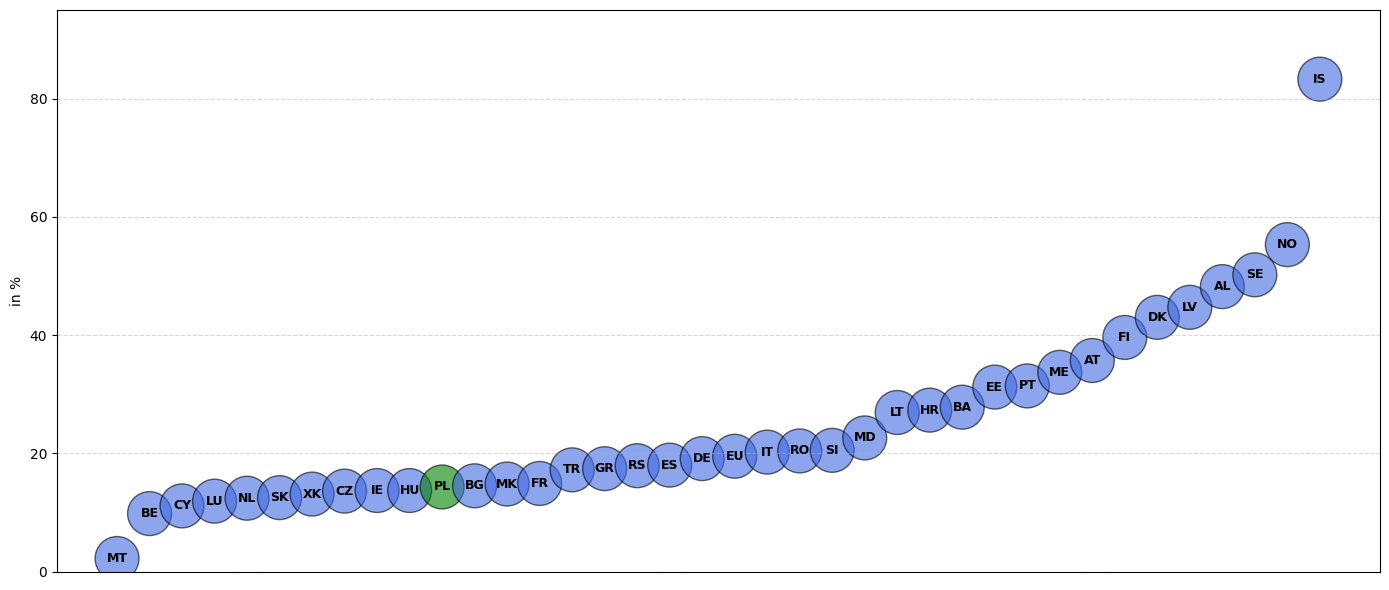
\includegraphics[width=\linewidth]{images/ozePercentageShare.png}
    \end{center}
\end{frame}

\begin{frame}
{Udział OZE i energii nuklearnej w sumarycznej produkcji energii wybranych krajów europejskich (2023)}
\begin{itemize}
    \item Pomimo bardzo dużego udziału OZE w sumarycznej mocy zainstalowanej Polski, realne wykorzystanie OZE w strukturze produkcji energii wynosi znacząco mniej.
    \item Polska posiada jeden z niższych procentowo udziałów OZE w realnej produkcji energii
    \item Największym udziałem OZE w strukturze energii cieszą się kraje o sprzyjających warunkach geograficznych.
    \item Wiele krajów łączy wykorzystywanie OZE z energią nuklearną.
    \end{itemize}
\end{frame}

\begin{frame}{Emisje CO\textsubscript{2} Per Capita (2023)}
    \includetable{co2_emissions}
\end{frame}

\begin{frame}{Cena energii dla gospodarstw domowych w Polsce na przestrzeni lat (zł, uwzględniając podatki)}
\begin{columns}

\begin{column}{0.6\textwidth}
        \includefigure{EnergyPriceOverYears}
\end{column}

\begin{column}{0.4\textwidth}
    \begin{itemize}
        \item Cena energii dla gospodarstw domowych przedstawia tendencję wzrostową.
        \item Najwyższa cena wśród lat 2020-2024 wystąpiła w roku 2024.
    \end{itemize}
\end{column}

\end{columns}
\end{frame}

\begin{frame}{Ceny energii dla gospodarstw domowych (PPS, uwzględniając podatki, 2023)}
    \includetable{energy_prices}
\end{frame}

\begin{frame}{Zależność energetyczna (2023)}
    \includetable{import_dependency}
%        \includefigure{test}
\end{frame}

%Tabela - ceny energii wybranych państw europejskichc w 2024
%jeszcze 1 tablea
%Mapka - kraje objęte OUTAGE
